\begin{figure}
    \centering
\begin{minipage}[t]{.19\textwidth}
\begin{subfigure}{\textwidth}
\centering
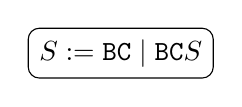
\begin{tikzpicture}[
box/.style={draw, rounded corners, minimum width=7cm, font=\sffamily},
]
    \node[box, inner sep=4pt, minimum height=0pt, minimum width=0pt] {
        $S := \texttt{BC} \mid \texttt{BC}S$
    };
\end{tikzpicture}
\caption{Example context-free grammar.}
\end{subfigure}

\begin{subfigure}{\textwidth}
\centering
\begin{tikzpicture}[
    box/.style={draw, rounded corners, font=\sffamily},
    tablebox/.style={draw, rounded corners, align=center, font=\sffamily},
    labelbox/.style={font=\bfseries\sffamily},
    every node/.style={outer sep=2pt}
]
   \node[state,initial above,initial text={}] (q_0) []  {$S_0$}; 
   \node[state] (q_1) [below=of q_0, xshift=-30pt] {$S_1$}; 
   \node[state,accepting] (q_2) [below=of q_0, xshift=30pt] {$S_2$}; 
   % \node[state] (q_4) [below=of q_3] {$q^{(}_4$};
   % \node[state] (q_5) [below=of q_4] {$q^{)}_5$};
    \path[->] 
    (q_0) edge node[above=10pt, pos=0.8] {\texttt{B}} (q_1)
    (q_1) edge node[above] {\texttt{C}} (q_2)
    (q_2) edge node[above=10pt, pos=0.2] {$\epsilon$} (q_0)
;

\end{tikzpicture}    
\caption{The corresponding automata for the context-free grammar.}
\end{subfigure}
\end{minipage}
\label{fig:grammar}
\end{figure}